\subsection{Frontend}\label{concept_fron}
Considering the frontend of the project first there has to be a design which fits to the requirements mentioned in the chapter \ref{reqfront}. This design shows in a more broad way how the features of showing AS-Pairs and adding AS-Pairs are implemented. \\

\subsubsection{Design Concept of the webpage}

\begin{figure}[H]
    \centering
    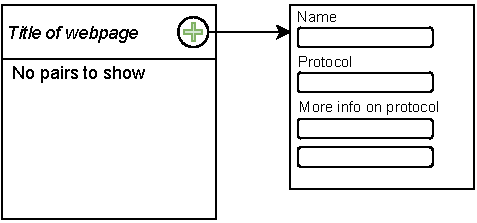
\includegraphics[width=.65\textwidth]{images/4_3/concept-webpage.pdf}
    \caption{Concept of the webpage}
    \label{fig:concept-webpage}
\end{figure}

Figure \ref{fig:concept-webpage} shows the concept of how the webpage should look like. The window on the left side is the first thing the user should see. It contains the title of the webpage, a plus sign button that holds the function to add pairs and the pairs that are in the database. For the case in figure \ref{fig:concept-webpage} there are no pairs in the database which is the reason why a default text is presented to the user informing him that no pairs are available. \\

If the user then clicks on the plus sign button it should bring up the window seen on the right side of figure \ref{fig:concept-webpage}. There information is needed from the user to be able to add an AS-Pair to the database. \\

The user has to first name the AS-Pair then the protocol has to be selected. In this case the protocol would be MQTT but the types of protocols can be anything an not only MQTT. To establish a connection between the AS-Pairs and the backend it is necessary to specify the IP of the broker and to which topic and subtopic the new AS-Pair belongs to. \newpage

\begin{wrapfigure}{L}{0.5\textwidth}
    \centering
     \begin{minipage}[b]{0.5\textwidth}
         \centering
         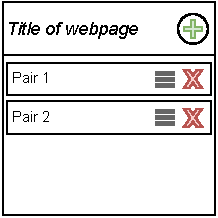
\includegraphics[width=\textwidth]{images/4_3/concept-webpage-pairs.pdf}
         \caption{Concept of the webpage with added AS-Pair}
         \label{fig:concept-webpage-pairs}
     \end{minipage}
  
\end{wrapfigure}

Only when the correct information has been entered by the user then it is possible to save the AS-Pair in the database. Which then would show up on the webpage. An example can be seen in the figure \ref{fig:concept-webpage-pairs} where pairs are available in the database. \\

As an addition there have been buttons added to delete a pair (red X button) and to show more information about the pair (three bars button) for further improvement of the webpage and the system interaction. But these buttons won't have any function for now as they are not important for the requirements. \\

\subsubsection{Realization of the Design Concept}

Now that the concept of the design is set it has to be realized. This is done through a JavaScript library called \textit{React.js}. Normally when building a user interface for a webpage it would need to implement HTML, CSS and JavaScript. With React the whole UI is made in one JavaScript file. That makes for a great benefit as it is now simpler to create an UI on a webpage. \\

Another benefit of React is that it optimizes the rendering of the web application which in turn has a benefit on the speed of the web application. This is done through taking the most recent domain object model (DOM) which is a tree like structure of all HTML-elements and creating a virtual DOM. When there are changes on the webpage it only compares the current state with the one that is saved as the virtual DOM. Then only the certain parts that are different will be rendered instead of calculating every CSS- and HTML-Element anew on the webpage when there have been changes made. \newpage

When creating the webpage as envisioned in the concept it is better to divide it into different parts as it reduces the complexity. These parts would for example be the \textit{Add-Button} or the \textit{Add-Pair-Form}. This is easily applicable in React and is even a feature that stands out as they are called components. Components are just reusable parts of the UI. \\

These components are separate JavaScript files that are then included in the main JavaScript file that renders the whole UI. Each of these components for the realization of the concept can be seen in figure \ref{fig:components} where they are highlighted.\\

\begin{wrapfigure}{r}{0.5\textwidth}
    \centering
     \begin{minipage}[b]{0.5\textwidth}
         \centering
         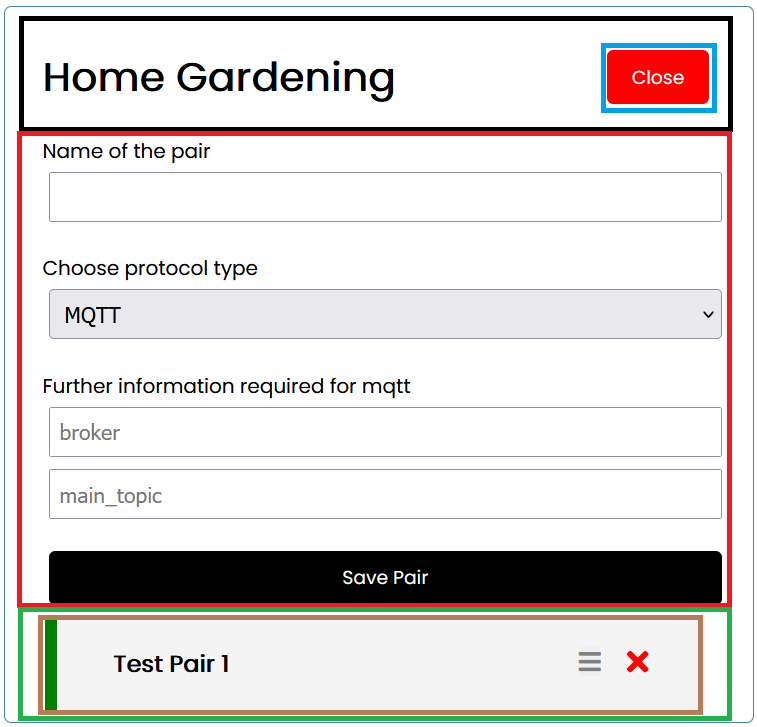
\includegraphics[width=\textwidth]{images/4_3/components.png}
         \caption{Components of the UI}
         \label{fig:components}
     \end{minipage}
     \vspace{-.25\baselineskip}
\end{wrapfigure}

The black border shows the \textit{header} component which contains the title of the page in this case \textit{Home Gardening} and the button component \textit{close}. The function of that button is to show and hide the form to add a new pair to the system. \\

With it being a component it is possible to pass so called properties, which are attributes that hold values. These props are used to change the color of the button or to change the text inside of it depending on if the form is shown or not. \\

Through the component highlighted in the red rectangle it is possible for the user to add a new pair. This component shows the user a form where different values are asked that resemble the idea in the conception of adding a new pair. \\

The name, protocol type and the information to connect to the protocol are needed which will be passed into a function in the main JavaScript file as a prop. This function handles the values received from the \textit{add-pair-form} component and passes them to the backend. \newpage

To pass values to the backend a POST-Request has to be made which is a HTTP-Request. This enables the communication between the server of the frontend and the server of the backend. \\

A successful communication is only possible if the user has stated the correct \textit{broker} and \textit{main topic} of the MQTT Protocol for example. To show the pairs that are available in the database the component in the green rectangle is created. That also contains another component for each individual pair. \\ 

To retrieve data about the pairs in the database and to display them on the webapp another HTTP-Request has to be done called \textit{GET}. These pairs are then saved in an object where through a \textit{map}-function every single pair is read and rendered onto the webpage as seen in the green rectangle in figure \ref{fig:components}. \\

\begin{figure}[H]
    \centering
    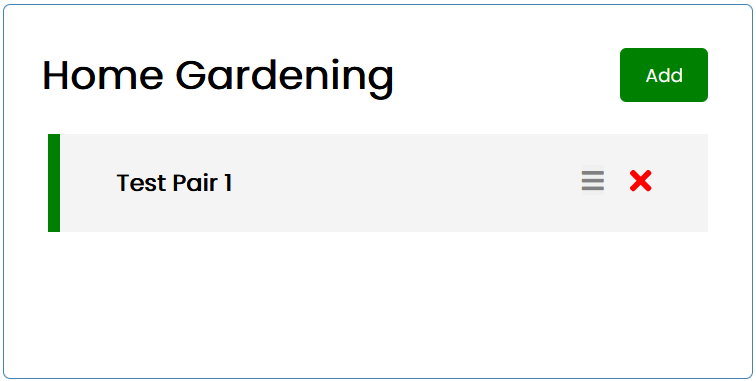
\includegraphics[width=.65\textwidth]{images/4_3/Screenshot 2021-07-27 095812.png}
    \caption{UI with an AS-Pair}
    \label{fig:UI-AS-Pair}
\end{figure}

Figure \ref{fig:UI-AS-Pair} shows how the webapp is rendered without the Add-Pair-Form being visible. Each pair shows the name of the pair and the status through the green bar on the left side of the pair. Additionally a \textit{red X button} and a button resembled by three bars are visible inside the pair component. \\

Even though the buttons are displayed they don't have any function but this satisfies the concept which also shows a \textit{red X button} and a \textit{three bars button}. These have already been implemented to later add a function to them.








